\documentclass[a4paper]{article}
\usepackage[utf8]{inputenc}
\usepackage[czech]{babel}
\usepackage[T1]{fontenc}

\usepackage[pdftex]{graphicx}
\usepackage{ifpdf}
\usepackage{hyperref}
\usepackage{tikz}

\usetikzlibrary{automata}

\title{Scrabble -- Programátorská dokumentace}

\author{Ondrej Profant}

\date{\today}

\ifpdf
\hypersetup{
	pdfauthor={Ondrej Profant},
	pdftitle={Scrabble -- Programátorská dokumentace},
	pdfsubject={Podrobná dokumentace k~programu Scrabble: http://github.com/Kedrigern/scrabble},
	pdfkeywords={scrabble, gaddag, trie, mono, monodevelop, csharp, gtk-sharp}
}
\fi

\begin{document}

\maketitle

\tableofcontents	

\newpage

%=================================
\section{Použité nástroje}
Program je psán v~jazyce C\# (verze 4) a využívá knihoven GTK\#. 
Pro vývoj bylo použito vývojové prostředí MonoDevelop (2.6) a distribuoaný systém správy verzí GIT (1.7.5.4).

Pro tvorbu grafiky Inkscape (0.48), externí dokumentace je psaná v~\LaTeX{u} (TeXLive 2009-13). Vyvíjeno na Ubuntu 11.04--11.10.



%=================================
\section{Zdrojové kódy -- obecně}
\subsection{Získání}
Příkazem:

\texttt{git clone git://github.com/Kedrigern/scrabble.git} 

\noindent
získáte celý projekt. Můžeme ho rozdělit do tří částí:
\begin{enumerate}
\item Scrabble: obsahuje samotný kód v~C\#. Soubory v~této složce uvidíte i z~Monodevelop, více viz kap. \ref{scrabble}.
\item scripts: Obsahuje pomocné skripty, více viz. podkapitola \ref{scripts}.
\item DOC-CS: Obsahuje dokumentaci (včetně \LaTeX{} zdrojových kódů)
\end{enumerate}

\subsection{Využití IDE}
Soubor s~koncovkou \texttt{sln} lze otevřít v~MonoDevelop, které vám zobrazí celou strukturu zdrojových kódů velmi přehledně.

Struktura rozdělení zdrojových kódů snad mluví sama za sebe. Většina důležitých tříd a funkcí je komentovaná přímo v~kódu -- velká část této dokumentace také vychází rovnou z~automaticky vyexportované inline dokumentace. 

Pokud by vám MonoDevelop nevyhovalo, tak můžeme bez problémů použít jinou strukturu (např. MS Visual Studio 2010 používá stejnou).

\subsection{Pomocné skripty}\label{scripts}
V~adresáři \texttt{scripts} je serie shellových skriptů, které pomáhají při kompilaci (např. různé druhy kompilace), balíčkování, získávání slovníků etc. 




%=================================
\section{Zdrojové kódy -- Scrabble}\label{scrabble}
\subsection{Obecně}
Základní běh programu se řídí tímto automatem:

\begin{tikzpicture}[shorten >=1pt,node distance=2.5cm]

\tikzstyle{every state}=[draw=black,very thick]

\node[state,initial] 		(q0) {\scriptsize{par}};
\node[state] 				(q1) [right of=q0] 		 {\scriptsize{InitWin}};
\node[state,accepting] 		(q2) [below of=q0]		 {\scriptsize{UnitTests}};
\node[state with output] 	(q3) [above right of=q1] {\scriptsize{MainWin} \nodepart{lower} \scriptsize{(client)}};
\node[state with output] 	(q4) [below right of=q1] {\scriptsize{MainWin} \nodepart{lower} \scriptsize{(general)}};
\node[state,accepting] 		(q5) [above right of=q4] {end};

\path[->] 	(q0) 	edge node [above left] {} (q1)
					edge node [below left] {\scriptsize{--test}} (q2)
					edge [loop above] node {\scriptsize{set vars}} ()
			(q1)	edge [loop above] node {\scriptsize{set vars}} ()
					edge node {} (q3)
					edge node {} (q4)
			(q3)	edge node [below right] {} (q5)
					edge [loop above] node {\scriptsize{iteration}} ()
			(q4)	edge node [below right] {} (q5)
					edge [loop below] node {\scriptsize{iteration}} ();	
\end{tikzpicture}

\subsection{GADDAG - motivace a popis}

Základní datová struktura a algoritmus je tak klíčová, že jí nejdříve popíšu poněkud obecněji, než je zvykem.

\subsubsection{Motivace}\begin{figure}[htb]
\centering
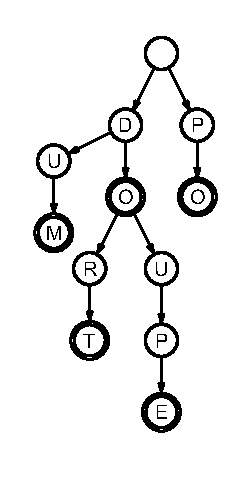
\includegraphics{pic/trie-all.pdf}
\caption{Trie pro slovník DŮM, DO, DORT, DOUPĚ, PO}
\label{trie}
\end{figure}
Základní klasickou reprezentací slovníku je Trie. V~anglickém slovníku o~94 240 slovech má trie 117 150 vrcholů a 179 618 hran. 

Existují metody, jak Trii komprimovat, např DAWG (Directed Acyclic Word-Graph), ale vzhledem k~dnešním počítačům mi to přijde až zbytečné (a to počítám i s~mobilními telefony). Na již zmíněném slovníku se dosáhne velikosti 175 KB oproti 780 KB v~normální Trii. Navíc je takováto reprezentace samozřejmě složitější a tím i náchylnější na chyby. 

Zajímavější je spíše Trii upravit k~našim algoritmickým potřebám. Budeme skládat slova dle modelu:\\
\texttt{PREFIX + JIŽ POLOŽENÁ PÍSMENA + SUFIX}

a potřebujeme tedy rychle (snadně) hledat prexfixy k~existujícím písmenům, abychom co nejméně omezily zcela nevhodná políčka. Obdobně třeba pracuje Boyer-Moorův vyhledávací algoritmus, který skáče v~textu na první pohled trochu nepřehledně, ale může tím ušetři značné prostředky.

\subsubsection{GADDAG}
 \begin{figure}[hb]
 \centering
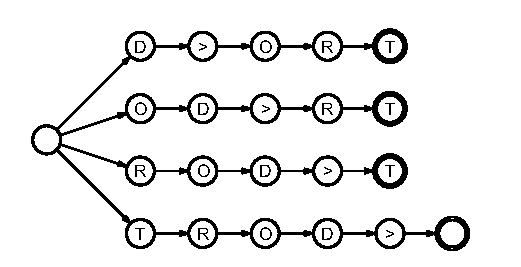
\includegraphics{pic/gaddag-dort.pdf}
\caption{GADDAG pro slovo DORT}
\label{gaddag-dort}
\end{figure}
Takovou reprezentaci v~roce 1993 představil Steven Gordon, nazval ji GADDAG. Tato struktura je podobná Trii (vychází z~ní), aby bylo možné v~ní rychle hledat. Slovo se zde dělí na všechny možné prefixy $x$ a zbytek $y$. Všechny možnosti jsou uloženy. Prefix je uložen zrcadlově, množinově zapsáno („>“ je pouze oddělovač):

$$\{ rev(x)>y\ |\ xy \mathrm{\ je\ slovo\ jazyka}\}$$

Díky tomu snadno analyzujeme zda se slovo na dané místo hracího plánu hodí. Nejdříve se totiž snažím pokládat prefix zprava doleva (obráceně než jsme zvyklí) a když narazíme na oddělovač, tak doplníme zbytek slova (na „druhém konci“). 

GADDAG pro jedno slovo délky $n$ má tedy $n$ cest, jak vidíme na obrázku \ref{gaddag-dort}, kde je celý GADDAG pro slovo DORT. Vidíme, že tato struktura je docela rozsáhla. Jaká je její velikost? V~případě anglického slovníku je přibližně $5\times$ větší než příslušná trie. Velikost se odvýjí od průměru délky slov ve slovníku, čili v~češtině bude velikost obdobná (ne o~moc větší).

\subsubsection{Algoritmus vyhledávání}
\begin{figure}[hb]
\centering
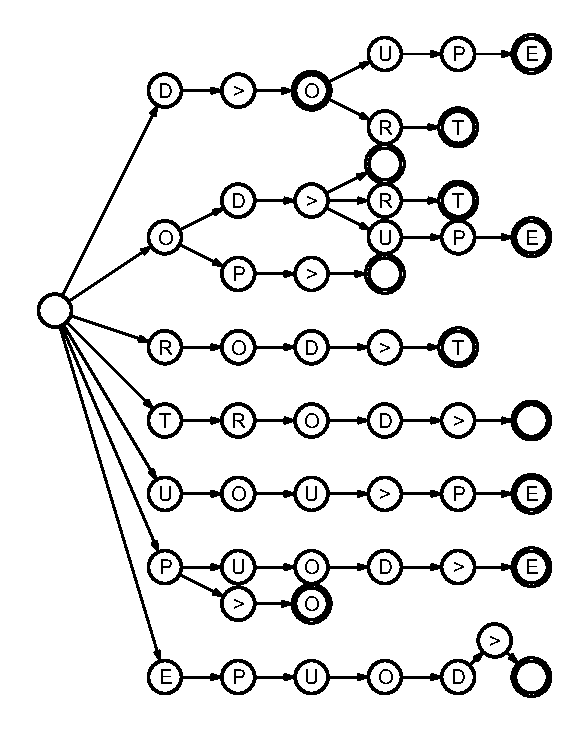
\includegraphics{pic/gaddag-all.pdf}
\caption{GADDAG pro slova DŮM, DO, DORT, DOUPĚ, PO}
\label{gaddag-all}
\end{figure}
V~našem slovníku budeme mít slova: DŮM, DO, DORT, DOUPĚ, PO.\footnote{V obrázcích je z~technických důvodů vynechána diakritika. Doufám, že to nepovede ke zmatení.} Slovník reprezentovaný trii je na obrázku \ref{trie}.

GADDAG pro slovo dort na obrázku \ref{gaddag-dort}. Jako oddělovač prefixu jsem zvolil ,,>''. Plný GADDAG pro náš slovník je na obrázku \ref{gaddag-all}.  


Pro jednoduchost zatím vynecháme zásobník (rack) a budeme předpokládat, že můžeme umístit libovolný počet libovolných písmen. Myslím, že je vidět, že zásobník následně poskytne jednoduchou heuristiku, která velmi ořeže možnosti.

Z~počátku budeme mít na naší hrací ploše slovo DŮM a DO (spojená skrz D). Plochu budeme procházet celou $2\times$. Prvně pro slova umístěná vodorovně (zleva doprava), podruhé pro slova umístěná zhora dolu.
\clearpage
\begin{verbatim}
     1 2 3 4 5 6        Procházení první:
    +-----------+        A1: Nemá spojení.
  A~|. . . . . .|        A2-3: Má spojení na B2, res B3 (popsáno dále)
  B |. D O~. . .|        A4-6: Nemá spojení.
  C |. Ů . . . .|        B1: Nemá spojení (připojení zleva se řeší z~druhé strany)
  D |. M . . . .|        B2-3: Obsazeno (přeskočíme)
    +-----------+        B4: Spojení skrz políčko vlevo - nejzajímavější situace.
\end{verbatim}
Při procházení nám zatím nastaly zajímavé situace na políčkách A2, A4 a B4. Na A2 začneme, zkoušíme vložit slovo zprava doleva (tak to umí GADDAG), čili projdeme první úroveň GADDAG a zjistíme, že písmena D, O, R, T, U, P, E mají sice návaznost (lze z~nich dále tvořit slovo), ale kontrolou křížení, zjistíme,  že ani jedno z~těchto písmen nemůžeme položit jako prefix slova DŮM.

U~A3 bude situace malinko jiná. Zjistíme, že můžeme položit D nebo P (slovo TO nemáme ve slovníku). Dokonce utvoří celá slova a tak spočítáme jejich hodnoty a uložíme je do možných řešení. Budeme dále postupovat zprava doleva na políčko A2, tentokrát, však budeme hledat slova začínající na D či P. Zde zjistíme, že kdybychom položili D, tak můžeme vpravo pokračovat slovami DOUPE a DORT. DOUPE by se nám nevešlo na hrací plán, ale DORT začínající na A3 je přípustným řešením. U~P zjistíme, že na A2 nemůžeme položit U. Nicméně druhá možnost položit P na A3 a O~na A4 lze -- máme další možné řešení.

Na B4 zjistíme reverzní prefix OD může vpravo pokrčovat na slova DORT a DOUPE (a že sám je slovem). A~máme další dvě slova do možných řešení. 

Zatím jsme vynechávali zásobník s~písmeny, které máme k~dispozici. Ten nám rozumně omezí možnosti i u~velkých plánů, Také jsme zjednodušili křížení, protože když položím písmeno, tak můžeme v~druhém směru také doplnit slovo.



\subsection{Podrobná dokumentace tříd}
Zde bych si dovolil odkázat na automaticky generovanou dokumentaci. 

Ve složce \texttt{scripts} najdete \texttt{makeDoc.sh}, který vám poskytne nejnovější verzi (vygenerována je do složky: \texttt{DOC-CS/htmldoc/}). 

Také je přístupná online (ne vždy aktuální):

\href{http://kedrigern.github.com/scrabble/doc}{http://kedrigern.github.com/scrabble/doc}

\section{Odkazy}
\begin{description}
\item[git]: \href{http://git-scm.com}{http://git-scm.com}
\item[GitHub]: \href{http://github.com}{http://github.com}
\item[GTK\#]: \href{http://www.mono-project.com/GtkSharp}{http://www.mono-project.com/GtkSharp}
\item[Inkscape]: \href{http://inkscape.org}{http://inkscape.org}
\item[Mono]: \href{http://www.mono-project.com}{http://www.mono-project.com}
\item[MonoDevelop]: \href{http://monodevelop.com}{http://monodevelop.com}
\end{description}

\end{document}
